\documentclass[12pt,twocolumn]{article}

% Page dimensions
\setlength{\hoffset}{-0.4in}
\setlength{\voffset}{-0.5in}
%\setlength{\headsep}{-0.2in}

\setlength{\oddsidemargin}{0in}
\setlength{\textwidth}{7.4in}
\setlength{\textheight}{8.5in}

\setlength{\columnsep}{0.3in}

% Packages
\usepackage{fancyhdr}
\usepackage{lastpage}
\usepackage{abstract}
\usepackage{amsmath, amssymb} 
\usepackage{epsfig}
\usepackage{subcaption} 
\usepackage[english]{alg}
\usepackage[usenames,dvipsnames]{color}
\usepackage{empheq}
%\usepackage[hidelinks]{hyperref}
\usepackage{hyperref}
\usepackage{sectsty}

\usepackage{morefloats}

% Packages for notes, testing, etc.
\usepackage{todonotes}
\usepackage[inline]{showlabels}

\showlabels[\color{blue}]{cite}
\showlabels[\color{blue}]{ref}

%% ============================================================

% Macros
\newcommand{\CHRONO}{{\sffamily{{Chrono}}}}
\newcommand{\ChronoFEA}{{\sffamily{Chrono}}::FEA}
\newcommand{\ChronoVehicle}{{\sffamily{Chrono}}::Vehicle}
\newcommand{\ChronoFSI}{{\sffamily{Chrono}}::FSI}
\newcommand{\ChronoGranular}{{\sffamily{Chrono}}::Granular}
\newcommand{\ChronoParallel}{{\sffamily{Chrono}}::Parallel}
\newcommand{\ChronoDistributed}{{\sffamily{Chrono}}::Distributed}
\newcommand{\ChronoOpenGL}{{\sffamily{Chrono}}::OpenGL}

%% ============================================================

% Styles

\definecolor{my-gray}{gray}{0.4}

% First page header
\fancypagestyle{firststyle} {
	\lhead{}
	\rhead{
	\footnotesize
	\textbf{2017 NDIA GROUND VEHICLE SYSTEMS ENGINEERING AND TECHNOLOGY SYMPOSIUM}\\
	\textbf{\sc Modeling \& Simulation, Testing and Validation (MSTV) Technical Session}\\
	\textbf{\sc August 8-10, 2017 -- Novi, Michigan}	
	}
	\chead{}
	%
	\lfoot{}
	\cfoot{}
	\rfoot{}
}

% All other pages (header and footer)
\pagestyle{fancy}
\fancyhf{}
\rhead{
	\color{my-gray}
	\footnotesize Proceedings of the 2017 Ground Vehicle Systems Engineering and Technology Symposium (GVSETS)
	}
\cfoot{
	\color{my-gray}
	\footnotesize
	{\FooterTitle}\\
	Page \thepage~of~\pageref{LastPage}
}

\renewcommand{\headrulewidth}{0pt}

% Font and styles for sections
\allsectionsfont{\fontsize{12}{15}\selectfont}

\renewcommand{\abstractname}{ABSTRACT}
\renewcommand{\refname}{REFERENCES}

%% ============================================================

\title{\bf\large PERFORMANCE ANALYSIS OF CONSTANT SPEED LOCAL OBSTACLE AVOIDANCE CONTROLLER USING AN MPC ALGORITHM ON GRANULAR TERRAIN}

\newcommand{\FooterTitle}{Performance analysis of obstacle avoidance algorithm on granular terrain}

\author{
	{\bf Nicholas Haraus}\\
	Dept. of Mechanical Engineering\\
	Marquette University\\
	Milwaukee, WI
	\and
	{\bf Radu Serban}\\
	Dept. of Mechanical Engineering\\
	University of Wisconsin - Madison\\
	Madison, WI
	\and
	{\bf Jonathan Fleischmann}\\
	Dept. of Mechanical Engineering\\
	Marquette University\\
	Milwaukee, WI
}

\newcommand{\MyAbstract}{
	A Model Predictive Control (MPC) Algorithm was used by Liu, Ersal, Stein, and Jayakumar~\cite{ModelFidelity2016} to develop a LIDAR-based constant speed local obstacle avoidance controller for autonomous ground vehicles. 
	When provided with LIDAR data as well as a target location, a vehicle can route itself around obstacles as it encounters them and arrive at an end goal via an optimal route.
	Using {\CHRONO}, a multibody physics API, this controller has been tested on a complex multibody physics HMMWV model to perform higher fidelity testing in more situations than previously accomplished. 
	For this research, the LIDAR-based constant speed local obstacle avoidance controller~\cite{ModelFidelity2016} has been implemented and tested on rigid flat terrain and granular terrain to examine the robustness of this control method. A novel simulation framework has been developed to efficiently simulate granular terrain for this application.
}

%% ============================================================

\begin{document}
\date{}

% Remove (comment) this block for final version
\tableofcontents
\thispagestyle{empty}
\newpage
\setcounter{page}{0}

% ------------------------------------------

\twocolumn[
\maketitle             % full width title
\thispagestyle{firststyle}
\begin{onecolabstract} % ditto abstract
\MyAbstract
\\\vspace{0.2in}
\end{onecolabstract}
]

%% ============================================================

\section{INTRODUCTION}\label{s:introduction}

Obstacle avoidance is a crucial capability for Autonomous Ground Vehicles (AGVs) of the future. This refers to a ground vehicle’s ability to sense its surrounding environment, develop an optimal path around the obstacles in the environment, generate optimal control commands to satisfy that path, and physically navigate the vehicle around the obstacles safely and to a desired endpoint. Safety is defined as avoiding collisions as well as enforcing limitations on excessive sideslip or tire lift-off. An ideal control algorithm is one that is capable of pushing a vehicle to its performance limits by using knowledge of its dynamic capabilities and surrounding environmental conditions while still enforcing the strict safety requirements. Though previous work has been accomplished testing a Model Predictive Control (MPC) algorithm for obstacle avoidance on wheeled vehicles, more work is required to test the fidelity of this algorithm and determine where improvements are needed. One area in which this algorithm has yet to be tested is its ability to control a wheeled vehicle on deformable terrain. Up to this point, the assumption that the terrain is rigid and flat for testing has been used. However, when rigid terrain is replaced with deformable terrain, such as soil or sand, how does the MPC algorithm perform?  Do the current most commonly used vehicle models perform successfully with the MPC algorithm on deformable terrain? The proposed research evaluates the robustness and validity of the MPC algorithm with different vehicle models in an environment more similar to what an off-road military vehicle would experience in combat. This testing is done via numerical simulation.

The goal of this paper is to present the results of this study to understand how model fidelity of the controller model affects overall performance of the obstacle avoidance controller. Certain challenges are introduced when attempting to simulate a vehicle on granular terrain: Specifically, how does the user efficiently allow the vehicle to drive everywhere without creating billions of particles scattered across the entire terrain? This challenge has been addressed by employing a simulation framework for granular terrain developed by the authors. The study has the following three objectives:
\begin{enumerate}
\item
Study and compare the performance of the MPC Controller on granular terrain compared to rigid terrain.
\item
Analyze the role of model fidelity of the internal controller model and how it affects the speed and performance of the obstacle avoidance controller.
\item
Showcase the potential of controller testing in a high fidelity virtual test environment with {\CHRONO} to assist with initial control algorithm development before physical implementation for vehicular applications.
\end{enumerate}

The remainder of this paper is organized as follows.  In Section~\ref{s:background} we provide overviews of the MPC based local obstacle avoidance algorithm, the {\CHRONO} multiphysics package used as the test environment. In Section~\ref{s:methodology} we describe the {\ChronoVehicle} HMMWV vehicle model used in this study as the plant model to be controlled and our proposed method for simulating a vehicle driving on deformable terrain over large distances. Then, the specific MPC LIDAR based local obstacle avoidance controller used for this study is presented. We introduce the different simplified lower fidelity analytical vehicle models used in the MPC algorithm to predict the /CHRONO vehicle behavior. We also provide descriptions of the test cases run for this study and a summary of the metrics used to compare performance of the various tested combinations. In Section~\ref{s:results} we presents the results of the tests outlined in the previous section as well as perform appropriate comparisons of the tests when the internal controller vehicle model is varied and when the terrain is changed from rigid to granular. Section~\ref{s:conclusion} wraps up the paper and presents potential future work based on the results of this study.

%% ============================================================

\section{BACKGROUND}\label{s:background}

\subsection{MPC Based Local Obstacle Avoidance }\label{MPC}

\begin{figure*}
	\centering
	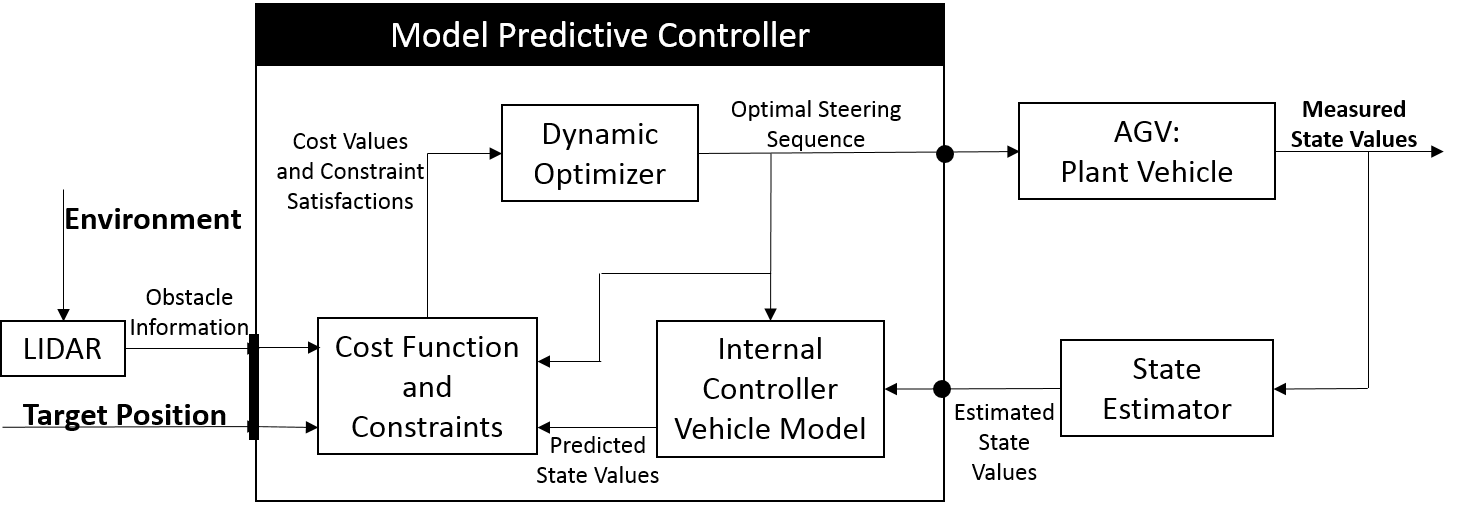
\includegraphics[width=0.6\textwidth]{Figs/MPCBlockDiagram.png}
	\caption{{\small Schematic of MPC LIDAR-Based Constant Speed Local Obstacle Avoidance Controller}}    
	\label{fig:MPC_schematic}
\end{figure*}

The concept of MPC is to use an internal model of the system one desires to control to predict and optimize future system behavior from the current system state and inputs. The system behavior is predicted over some defined finite time horizon and the optimal control sequence over the prediction horizon is output. The control sequence is executed for an execution time smaller than the prediction horizon, and the whole process is repeated. The repetition of this process over time creates a feedback loop which continually controls the system, pushing it towards an optimal path.

For this study, the system to be controlled is an AGV. Consider an AGV located in a level environment without roads or any other structures to guide the AGV’s motion. The AGV also has a known global target position. Between the target position and the current vehicle position there may or may not be obstacles of unknown size. Using the MPC formulation outlined in~\cite{ModelFidelity2016}, the vehicle can navigate from the current position to the provided target position while avoiding obstacles as they are encountered. Obstacle information is assumed to be unknown a priori and only obtained through a planar LIDAR sensor. The MPC schematic is presented in Fig.~\ref{fig:MPC_schematic}.
%

\begin{figure}
	\centering
	\begin{subfigure}[b]{\columnwidth}
		\centering
		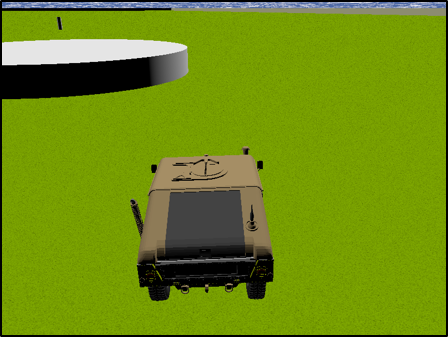
\includegraphics[width=0.8\columnwidth]{Figs/incomingObst.png}
		\caption{{\small 3D Visualization of LIDAR Encountering Obstacle}}   
		\label{fig:obstacle_field_3D}
	\end{subfigure}

	\hfill
	\begin{subfigure}[b]{\columnwidth}
		\centering
		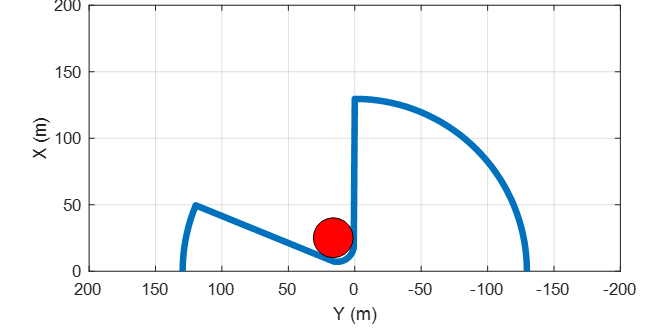
\includegraphics[width=\columnwidth]{Figs/obstLIDAR.png}
		\caption{\small LIDAR Sensed Safe Area}   
		\label{fig:obstacle_field_LIDAR}
	\end{subfigure}
	\caption{\small Sample obstacle field and LIDAR output}
	\label{fig:LIDARExample}
\end{figure}

The planar LIDAR sensor is mounted at the front center location of the vehicle. The LIDAR sensor returns the closest obstacle boundary in all radial directions of the sensor at an angular resolution ε. The LIDAR sensor has a maximum range past which it cannot sense any obstacles. Therefore, if the closest obstacle boundary is greater than the LIDAR radius $R_{LIDAR}$ then the sensor returns $R_{LIDAR}$. The LIDAR sensor range is [$0^\circ$, $180^\circ$] with $90^\circ$ being the vehicle heading direction. Since for this study the AGV is driving along level ground, whether granular or rigid, the planar LIDAR sensor is sufficient. The LIDAR is assumed to have no delay and zero noise. Therefore, the LIDAR sensor can instantaneously generate a safe area polygon assembled from the returned points from the LIDAR. An overhead view of the AGV encountering an obstacle and the generated LIDAR safe area polygon are presented in Fig.~\ref{fig:LIDARExample}. 
%

The outputs of the MPC algorithm are the steering signals only for this simulation. As shown in Fig.~\ref{fig:MPC_schematic}, the MPC algorithm is made up of the internal controller vehicle model, the cost function and constraints, and the dynamic optimizer. The internal controller vehicle model predicts the future states of the AGV for a given steering sequence and is of interest in this work. For this study, the internal controller vehicle model is varied from test to test between a 2-DOF vehicle model and a 14-DOF vehicle model, detailed in further sections. The cost functions and constraints are used to formulate the optimal control problem with the equations from the vehicle model. The dynamic optimizer then solves the optimal control problem. For the purpose of this paper, exhaustive search is used to find the optimal solution to the problem since solution speed is not a primary focus of this paper, but more importantly the ability to find and execute an optimal solution. With this method, the steering sequence is discretized and a finite of path possibilities are tested and weighed by a cost function. 

%% ============================================================

\subsection{{\CHRONO} Multibody Physics Package}\label{ss:Chrono}

The physics modeling and simulation capabilities are provided by the multiphysics open-source package {\CHRONO}~\cite{Chrono2016}. The core functionality of {\CHRONO} provides support for the modeling, simulation, and visualization of rigid multibody systems, with additional capabilities offered through optional modules. These modules provide support for additional classes of problems (e.g., finite element analysis and fluid-solid interaction), for modeling and simulation of specialized systems (such as ground vehicles and granular dynamics problems), or provide specialized parallel computing algorithms (multi-core, GPU, and distributed) for large-scale simulations.

%% ------------------------------------------------------------

\subsubsection{Vehicle Modeling}\label{sss:Chrono_Vehicle}
	
Built as a {\CHRONO} extension module, {\ChronoVehicle}~\cite{ChronoVehicle_TR} is a C++ middleware library focused on the modeling, simulation, and visualization of ground vehicles.
%
{\ChronoVehicle} provides a collection of templates for various topologies of both wheeled and tracked vehicle subsystems, as well as support for modeling of rigid, flexible, and granular terrain, support for closed-loop and interactive driver models, and run-time and off-line visualization of simulation results.

Modeling of vehicle systems is done in a modular fashion, with a vehicle defined as an assembly of instances of various subsystems (suspension, steering, driveline, etc.).  Flexibility in modeling is provided by adopting a template-based design. In {\ChronoVehicle}, templates are parameterized models that define a particular implementation of a vehicle subsystem. As such, a template defines the basic modeling elements (bodies, joints, force elements), imposes the subsystem topology, prescribes the design parameters, and implements the common functionality for a given type of subsystem (e.g., suspension) particularized to a specific template (e.g., double wishbone). Finally, an instantiation of such a template is obtained by specifying the template parameters (hardpoints, joint directions, inertial properties, contact material properties, etc.) for a concrete vehicle (e.g., the HMMWV front suspension).

For wheeled vehicle systems, templates are provided for the following subsystems:
{\em suspension} (double wishbone, reduced double wishbone using distance constraints, multi-link, solid-axle, McPhearson strut, semi-trailing arm);
{\em steering} (Pitman arm, rack-and-pinion);
{\em driveline} (2WD and 4WD shaft-based using specialized {\CHRONO} modeling elements, simplified kinematic driveline);
{\em wheel} (simply a carrier for additional mass and inertia appended to the suspension's spindle body);
{\em brake} (simple model using a constant torque modulated by the driver braking input).

In addition, {\ChronoVehicle} offers a variety of tire models and associated templates, ranging from rigid tires, to empirical and semi-empirical models (such as Pacejka and Fiala), to fully deformable tires modeled with finite elements (using either an Absolute Nodal Coordinate Formulation or a co-rotational formulation).  Driver inputs (steering, throttle, and braking) are provided from a {\em driver} subsystem with available options in {ChronoVehicle} including both open-loop (interactive or data-driven) and closed-loop (e.g., path-following based on PID controllers).

%% ------------------------------------------------------------

\subsubsection{Granular Mechanics}\label{sss:GranMech}

In this work, the focus is on modeling and simulating the terrain and the tire-terrain interaction using high-fidelity, fully-resolved granular dynamics simulations, employing the Discrete element Method (DEM).  Meaningful mobility simulations require large enough terrain patches and small enough particle dimensions that result in DEM problems involving frictional contact with millions of degrees of freedom.

Unlike continuum-based deformable terrain modeling approaches, DEM treats all component particles separately, as distinct entities, by maintaining and advancing in time their states while taking into account pair-wise interaction forces due to frictional contact.
%
Broadly speaking, computational methods for DEM at this scale can be categorized into two classes: penalty-based (also known as a compliant-body approach; denoted here by DEM-P) and complementarity-based (also known as a rigid-body approach; denoted here by DEM-C).  While differing in the underlying formulation employed for modeling and generating the normal and tangential forces at the contact interface, and thus leading to different mathematical models and different problem sizes, both methods rely crucially on efficient methods for proximity calculation. This common algorithmic step provides a complete geometric characterization of the interaction between neighboring bodies, taking into account the current system state and specification of the contact shapes associated with all interacting bodies. For this study, the penalty based DEM-P approach is used.

Penalty methods begin with a relaxation of the rigid body assumption~\cite{cundall71}. A regularization approach, DEM-P assumes local body deformation at the contact point. Employing the finite element method to characterize this deformation would incur a stiff computational cost. Instead, an approximation is employed, using information generated during the collision detection stage of the solution, and the local body deformation is related to the depth of inter-penetration between two otherwise rigid contact shapes. In order to apply results from Hertz contact theory, valid for sphere-sphere interactions, the contact shapes are further approximated by their local radius of curvature at the contact point~\cite{johnson1987contact}.
%
This approach yields a general methodology for computing the normal and tangential forces at the contact point.   For granular dynamics via DEM-P, the equations of motion need not be changed. Indeed, normal and tangential contact forces are treated as any external forces and directly factored in the momentum balance.
%
For details on the specific DEM-P implementation in {\CHRONO}, see~\cite{fleischmannetalJCND2015}.
%
In this work, we employed the DEM-P capabilities in {\CHRONO}, leveraging the multi-core, OpenMP-based parallelization features offered by the {\ChronoParallel} module.  

%%============================================================

\section{TECHNICAL APPROACH AND METHODOLOGY}\label{s:methodology}

\subsection{Full-Vehicle Multibody Model}\label{ss:FullVehicleModel}

The model to be controlled (the {\em plant}) is a full-vehicle {\ChronoVehicle} model of an HMMWV, which includes multi-body subsystems for the suspensions, steering, driveline, and powertrain, and is available in the {\CHRONO} package.

This vehicle model (see Fig.~\ref{fig:hmmwv}) has a curb weight of $2,550$~kg.
%
It includes independent front and rear double wishbone suspensions and a Pitman arm steering mechanism. The shock absorber and coil spring, mounted between the lower control arm and the chassis, are modeled with {\CHRONO} nonlinear force elements and include the effects of bump stops.
%
\begin{figure}
	\centering
	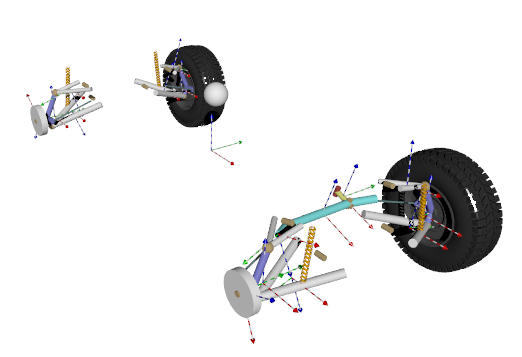
\includegraphics[width=\columnwidth]{Figs/hmmwv_bodies.png}
	\caption{\small Full-vehicle HMMWV multibody model.}  
	\label{fig:hmmwv}
\end{figure}

The AWD driveline is modeled using {\CHRONO} shaft elements and includes three power splitting elements (a central differential and front/rear differentials), as well as conical gears connected through 1-dimensional shaft elements which carry rotational inertia. 
%
The powertrain is also modeled using 1-dimensional shaft elements and includes models for a thermal engine specified through speed-torque maps for power and engine losses, a torque converter specified via maps for the capacity factor and the torque ratio, and an automatic transmission gearbox with three forward gears and a single reverse gear.
%
The connection between powertrain and driveline is a force-displacement interface at the driveshaft (with torque applied from the powertrain and angular velocity provided by the driveline).

For mobility studies on deformable terrain, provided that the tire inflation pressure is comparable or larger than the average ground pressure, according to the postulate by Wong~\cite{wong93} the tire can be considered in a so-called {\em rigid regime}.  As such, tire deformation can be ignored and the vehicle's tires modeled using rigid contact shapes.  The HMMWV tire model used here is thus represented by a cylinder with a radius of $0.47$~m ($18.5$~in) and a width of $0.254$~m ($10$~in).


%% ============================================================

\subsection{Relocating Granular Patch }\label{ss:Patch}

Due to the large-scale nature of the simulations in this study, generating granular particles scattered across the whole obstacle field to simulate granular terrain is both computationally exhausting and unreasonable. The computational times to complete a simulation of this sort of scale would be too large to justify the completion of this sort of study. Instead, a mechanism has been developed for this study to address the issue of scale when simulating a ground vehicle traversing over a large granular terrain. Consider an AGV on a large granular terrain of $100$ by $100$ meters. Since we are primarily interested in the behavior of the vehicle on the terrain and not specifically the terrain behavior itself, we assume only a small patch of granular terrain underneath and around the vehicle actually has a significant effect on vehicle behavior and performance. This idea promoted the development of a relocating granular patch used for this study to allow a vehicle to traverse granular terrain over a large-scale area without the need to generate particles everywhere throughout the terrain area. 

\begin{figure}
	\centering
	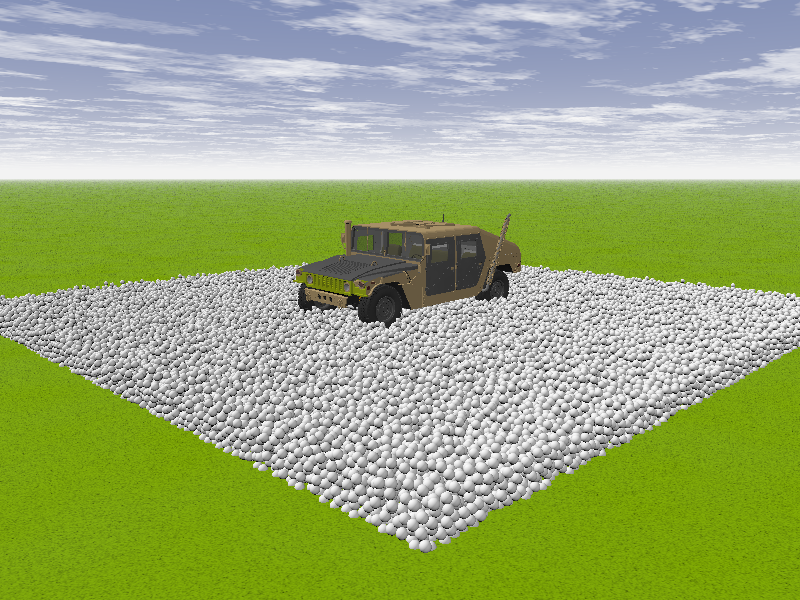
\includegraphics[width=0.8\columnwidth]{Figs/granPatch.png}
	\caption{\small Relocating Granular Patch that follows the vehicle}  
	\label{fig:granPatch}
\end{figure}

This mechanism allows a user to generate granular particles within a specified distance of the vehicle's CoG. Figure~\ref{fig:granPatch} presents the patch of granular terrain underneath the {\CHRONO}  HMMWV that will allow follow the HMMWV. The particles are contained within four rigid walls to prevent particles from escaping the desired terrain area. As the vehicle moves across the terrain, this granular patch maintains granular terrain underneath the vehicle by consistently relocating particles as the become too far away from the vehicle. When the vehicle CoG comes within a certain distance of any of the walls, a band of particles from the opposite end of the granular patch are relocated past the closest wall and all of the walls are shifted in that direction. Each of these relocation steps keeps the vehicle on top of granular terrain at all times. Depending on the vehicle, this granular patch can be resized for both computationally efficiency and to guarantee the vehicle maintains a reasonable distance from the walls to prevent any edge effects. This newly developed method of simulating granular terrain for AGV's is omnidirectional in the ground plane, allowing the vehicle to move in any direction while the terrain patch relocates and responds to that movement. This method of granular terrain mobility allows the user to specify parameters of the particles and thus allows for simulation of a vehicle over a largely customizable flat terrain.

For our simulations, the granular patch was maintained at a size of roughly $6.6$ by $6.6$ meters.  This number was assigned as two times the largest dimension of the vehicle, which in the case of the HMMWV is $3.3$~m (in length).  The dimensions of the patch are not constant, however, since the patch expands in the direction of relocation by two times the largest particle radius every time the advancing wall is shifted.  This is done in order to avoid particle overlap, since the relocated particles are moved to a position that is shifted one largest particle radius ahead of the particles adjacent to the advancing wall.  After relocation, the walls of the granular patch are given a recovery velocity such that the granular patch regains its original dimensions in $0.1$ seconds.  This recovery time should be small relative to the duration of the simulations, and in general it will also depend on the velocity of the vehicle, since the granular patch should completely recover its dimensions between subsequent relocations.

Within the granular patch, the granular terrain was modeled by $55,931$ uniform spherical particles, with a micro-scale inter-particle sliding friction coefficient of $\mu = 0.8$, and particle diameter of $0.1$~m.  Previous studies \cite{fleischmannetalGEGE2014} have shown that 
a randomly packed assembly of as few as $3,000$ - $30,000$ uniform spheres will exhibit macro-scale bulk granular material yield behavior (due to inter-particle sliding) that closely matches the Lade-Duncan yield surface, which is a well-established yield criterion in the field of geomechanics, where the macro-scale friction angle $\phi$ for the bulk granular material can be determined as a function of the inter-particle friction coefficient $\mu$.

Referring to Fig.~10 of \cite{fleischmannetalGEGE2014}, a randomly packed assembly of uniform spheres with an inter-particle friction coefficient of $\mu = 0.8$ will exhibit macro-scale yield behavior corresponding to a bulk granular material with a macro-scale friction angle between roughly $35^\circ \leq \phi \leq 40^\circ$ if particle rotation is allowed (6 DOF particles), or with a macro-scale friction angle between roughly $65^\circ \leq \phi \leq 70^\circ$ if particle rotation is prohibited (3 DOF particles).
%
Since the granular patch used in our simulations contains more than $50,000$ uniform spheres, we can reliably conclude that our granular patch is accurately modeling the yield behavior of a true granular material on the macro-scale: either with a macro-scale friction angle of $35^\circ-40^\circ$ if particle rotation is allowed, which is typical of a wide range of dry natural and crushed sands \cite{Cho&Dodds&Santamarina2006}; or with a macro-scale friction angle of $65^\circ-70^\circ$ if particle rotation is prohibited, which is typical of crushed or fragmented rock, such as railway track ballast \cite{Indraratnaetal1998}.

% NOTE: THE WORDING OF THE FOLLOWING WILL CHANGE FOR THE FINAL DRAFT!!!
In this first draft of our paper, we only include simulation results for the granular material model corresponding to a macro-scale or bulk material friction angle of $65^\circ-70^\circ$ (using 3 DOF particles), which essentially models a field of fragmented rock.  In the final draft of this paper, we will also include simulation results for the granular material model corresponding to a macro-scale bulk friction angle of $35^\circ-40^\circ$ (using 6 DOF particles), which models dry sand.  Thus, in the final draft of this paper, we will compare the MPC algorithm performance on both fragmented rock and dry sand, as well as on rigid terrain.

We note that in the case of the HMMWV, the vehicle tire width is equal to only approximately $2.5$ particle diameters in the granular patch.  This is less than ideal.  However, a more ideal value of $10$ particle diameters per tire width would increase the number of particles in the granular patch to more than $3$ million, which would result in prohibitively slow simulations, particularly for events corresponding to physical time durations on the order of $10$ seconds or more.

%%============================================================

\subsection{{\CHRONO} Multibody Physics Package}\label{ss:Chrono}

The physics modeling and simulation capabilities are provided by the multiphysics open-source package {\CHRONO}~\cite{Chrono2016}. The core functionality of {\CHRONO} provides support for the modeling, simulation, and visualization of rigid multibody systems, with additional capabilities offered through optional modules. These modules provide support for additional classes of problems (e.g., finite element analysis and fluid-solid interaction), for modeling and simulation of specialized systems (such as ground vehicles and granular dynamics problems), or provide specialized parallel computing algorithms (multi-core, GPU, and distributed) for large-scale simulations.
%%============================================================

\subsection{Implemented MPC LIDAR Based Local Obstacle Avoidance}\label{ss:MPCImplementation}

The MPC controller as formulated in~\cite{ModelFidelity2016} is used for this study. The cost function and constraints need to be specified to avoid collisions with obstacles and guarantee vehicle dynamical safety. The optimal control problem solved at each MPC time step is comprised of the following set of equations:

\begin{equation}\label{e:MPCCost}
J = s_T + wd 
\end{equation}
\begin{equation}\label{e:State_ODE}
\dot{\xi} = v\left[\xi\left(t\right),\zeta\left(t\right)\right] 
\end{equation}
\begin{equation}\label{e:InitialStates}
\xi\left(0\right) = \xi_0 
\end{equation}
\begin{equation}\label{e:SafeArea}
\tilde{S}\left[x\left(t\right),y\left(t\right)\right] \leq0  
\end{equation}
\begin{equation}\label{e:SteerLimit}
\left|\delta_f\left(t\right)\right| \leq\tilde{\delta}_{f,max}\left(U_0\right) 
\end{equation}
\begin{equation}\label{e:SteerRateLimit}
\left|\varsigma_f\left(t\right)\right| \leq\varsigma_{f,max} 
\end{equation}
\begin{equation}\label{e:TimeDomain}
t \in \left[0,T_P\right]
\end{equation}

Equation~(\ref{e:MPCCost}) defines the cost function for this optimal control problem. This equation is a soft requirement which defines how the separate path possibilities are weighed against each other and how to determine which path is actually optimal. The cost function is comprised of two terms defined by the following
%
\begin{equation}\label{e:DistanceCost}
s_T = \sqrt{\left[ x_G - x\left(T_P\right)\right]^2 + \left[y_G - y\left(T_P\right)\right]^2 }
\end{equation}
\begin{equation}\label{e:TurningCost}
d = \int \limits_0^{T_G} \left|\varsigma\left(t\right)\right| dt 
\end{equation}
%
$s_{T}$ seeks to minimize the distance between the prediction end location and the target position. A prediction path that guides the vehicle to the closest location to the target will have the smaller $s_{T}$ term. The second term $d$ aims to minimize the change in steering angle so that smoother, straighter paths are more favorable than windy paths. A weighting factor $w$ is used to scale the influence of $d$ on the total cost.

Equations~(\ref{e:State_ODE}-\ref{e:TimeDomain}) are the constraint equations for this optimal control problem which represent hard requirements for vehicle safety and avoiding collisions. Any paths that violate these constraints are not considered safe paths and are eliminated as potential options in this prediction window. Equation~(\ref{e:State_ODE}) defines a set of differential equations that describe the internal controller vehicle model. These equations are presented further in the paper or left for formulation in references. Equation~(\ref{e:InitialStates}) presents the initial states needed to solve Eq.~(\ref{e:State_ODE}) for potential paths. 

Equation~(\ref{e:SafeArea}) defines a safe area polygon. All points along paths found from Eqs.~(\ref{e:State_ODE})-(\ref{e:InitialStates}) must fall inside of this safe area polygon. This safe area is constructed from LIDAR points. An additional safety buffer is added to account for vehicle size and prevent corners of the vehicle from colliding with an obstacle. 

Equation~(\ref{e:SteerLimit}) imposes a limit on maximum steering angle for the vehicle based on vehicle speed. This value is obtained from a lookup table which can be generated either experimentally or from simulation. Equation~(\ref{e:SteerRateLimit}) imposes a maximum limit on steering rate. Equation~(\ref{e:TimeDomain}) defines the time limits over which this optimal control problem is solved.

Equation ~(\ref{e:State_ODE}) as noted above refers to an analytical vehicle model expressed as a set of differential equations. This is how the controller is able to predict vehicle performance within the prediction horizon. The accuracy of the internal vehicle controller model should directly influence the driven vehicle's controlled performance. If the internal vehicle controller model poorly predicts a vehicle's response to inputs from the driver or the environment, then these deficciencies will be witnessed when attempting to control the driven vehicle. In the case of this study, an internal vehicle controller model that poorly represents the driven vehicle may predict that a specified steering sequence will navigate the driven vehicle around an approaching obstacle, but due to this descrepancy the driven vehicle may not turn quickly enough and collide with the obstacle. However, using an internal vehicle controller model that is highly complex may provide accurate trajectory and vehicle response predictions, but the time required to solve an optimal control problem with this complicated set of differential equations is much higher than using a simpler internal vehicle controller model. Since the eventual goal is physical implementation of this controller, an ideal controller would not just accurately predict vehicle responses but also do it quick enough to insure vehicle safety. Therefore for this study the driven vehicle that will be controlled is a HMMWV developed in {\CHRONO}.  This vehicle will be controlled using two separately developed controllers. The first controller uses a simple 2-DOF vehicle model to predict the {\CHRONO}  HMMWV trajectory for different series of steering sequences and is presented in detail in Section~\ref{sss:2DOFModel}. The second controller uses a complex 14-DOF vehicle model to predict vehicle states for different series of steering sequences. Once again, this study will test each of these controller's abilities to successfully navigate the driven {\CHRONO}  HMMWV vehicle through two obstacle fields on rigid flat terrain and then granular terrain. The driven {\CHRONO} HMMWV vehicle is presented in detail in Section~\ref{ss:FullVehicleModel}. Exhaustive search space is used to solve the optimal control problem in each time step since the goal of this study is to analyze the vehicle's ability to be successfully navigated through an obstacle field and not how quickly the problem can be solved. A sample visualization of the different predicted trajectories from the 2-DOF model is presented in Fig.~\ref{fig:PossiblePaths}. A point in polygon algorithm is used to determine which trajectories remain inside of the safe area polygon visualized in Fig.~\ref{fig:LIDARExample} and therefore should be compared to the other possibilities using Eq.~(\ref{e:MPCCost}).

\begin{figure}
	\centering
	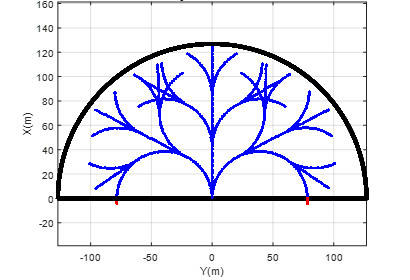
\includegraphics[width=\columnwidth]{Figs/PathPossibilities.png}
	\caption{\small Potential Paths predicted by 2-DOF Internal Vehicle Controller Model}  
	\label{fig:PossiblePaths}
\end{figure}

An exhaustive search method is used for this study as the dynamic optimizer since the goal of this study is to identify the controller's ability to identify the best solution instead of analyzing how quickly that solution is found~\cite{ModelFidelity2016}. The steering space is discretized into five possible steering angles. The prediction horizon is split into four intervals. This results in 625 different steering sequence possibilities and therefore 625 different path possibilities each controller time step that are wieghed by the controller to determine which steering sequence and resulting path forward is best. This concept is visualized in~ref{fig:PossiblePaths} with only three steering angles considered over three intervals for visualization purposes.

%% ============================================================

\subsection{Internal Controller Vehicle Models}\label{ss:IntModel}

The vehicle models embedded in the MPC are simplifications of the full, multi-body based, {\CHRONO} wheeled vehicle model which is being controlled.  We consider two such models, providing different levels of fidelity, as described below.

%% ------------------------------------------------------------

\subsubsection{Two DOF Vehicle Model}\label{sss:2DOFModel}
The standard vehicle model used in newly developed MPC obstacle avoidance algorithms such as~\cite{ModelFidelity2016} is the 2-DOF yaw plane vehicle model. These models normally either assume constant cornering stiffness or the nonlinear Pacejka Magic Formula Tire Model~\cite{foo} to predict the ground tire interaction forces. For this study and due to the availability of experimental data, the Pacejka Magic Formula is used to predict tire forces in the vehicle models.   

A visual representation of the 2-DOF yaw plane vehicle model can be found in Fig.~\ref{fig:2DOF}. The 2-DOF model is described by the following first-order ordinary differential equations:

\begin{equation}\label{e:2DOF_Vdot}
\dot{V} = \left(F_{y,f} + F_{y,r}\right)/{M - U_0r} 
\end{equation}
\begin{equation}\label{e:2DOF_rdot}
\dot{r} = \left(F_{y,f} - F_{y,r}\right)/I_{zz}
\end{equation}
\begin{equation}\label{e:2DOF_psidot}
\dot{\psi} = r 
\end{equation}
\begin{equation}\label{e:2DOF_xdot}
\dot{x} = U_0\cos{\psi}-\left(V+L_fr\right)\sin{\psi}
\end{equation}
\begin{equation}\label{e:2DOF_ydot}
\dot{y} = U_0\sin{\psi}+\left(V+L_fr\right)\cos{\psi} \,,
\end{equation}
%
where $F_{y,f}$ and $F_{y,r}$ are the lateral tire forces at the front and rear axles, respectively. $U_0$ and $V$ are the longitudinal speed and lateral speed of the vehicle in the vehicle’s coordinate frame. $\psi$ is the yaw angle and $r$ is the yaw rate. $\left(x,y\right)$ represent the front center location of the vehicle expressed in global coordinates. $M$ is vehicle mass, $I_{zz}$ is the moment of inertia of the vehicle, $L_f$ is the distance from the front axle to the vehicle CoG, and $L_r$ is the distance from the rear axle to the vehicle CoG. For this study, the model is constrained to a constant longitudinal speed. Then the planar 3-DOF body with one constraint results in the 2-DOF model used for this study.

\begin{figure}
	\centering
	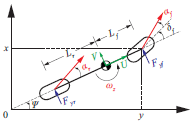
\includegraphics[width=0.8\columnwidth]{Figs/2DOF_Stein.png}
	\caption{\small 2-DOF Vehicle Model \cite{ModelFidelity2016}}  
	\label{fig:2DOF}
\end{figure}

%% ------------------------------------------------------------

\subsubsection{Fourteen DOF Vehicle Model}\label{sss:14DOFModel}
A 14-DOF model is often used in studies such as these to test the obstacle avoidance controller with a higher fidelity vehicle model~\cite{ModelFidelity2016, ModelFidelity2013}. A benefit of using the 14-DOF in the controller is the model’s ability to predict tire liftoff and account for dynamic effects from suspension systems. For this paper then it is appropriate to also compare performance of the local obstacle avoidance controller running an internal fourteen DOF on rigid terrain versus granular terrain.  

The 14-DOF vehicle model consists of one sprung mass connected above four unsprung masses~\cite{RollStudies2007}. The sprung mass is allowed to roll, pitch, and yaw while also displacing laterally, vertically, and longitudinally. This sprung mass contributes six DOF to the model. Each of the four wheels are allowed to bounce vertically and rotate about the wheel horizontal axis. The front two wheels are also free to steer. Each wheel then contributes two DOF to the fourteen DOF model. The model is constrained at a constant longitudinal speed. The equations used for this model as well as their developments can be found in~\cite{RollStudies2007}.

%% ============================================================
%\subsection{Open Loop Comparisons }\label{ss:OpenLoop}

%% ============================================================

\subsection{Evaluation Metrics}\label{ss:Metrics}
Five evaluation metrics will be used to compare one test performance to the other. First, all test runs will be compared based on the time to reach the target $T_{target}$. Tests on the same terrain can be compared with this metric to determine which controller leads the vehicle to the target point quickest. Second, the closest distance the vehicle reaches to any obstacle $d_{min}$ will be measured. A controller that accurately predicts vehicle performance should allow the vehicle get much closer to obstacles. Third, the control effort will be calculated and compared between test cases. Fourth, the max lateral acceleration of the vehicle will be determined. Finally, the average lateral acceleration will be determined from the test cases. Using the DEM-P method of simulation results in noisy acceleration data. To address this, acceleration data is filtered to remove noise. The accelerations are calculated at the driver's position in the chassis. These five evaluation metrics provide a logical method for comparing one test case to another whether two test cases are on different terrain, have different analytical controller models, or both. 

%% ============================================================

\subsection{Numerical Simulation Setup }\label{ss:Setup}

\begin{table}
\begin{center}
	\begin{tabular}{||c |c | c||} 
		\hline
		Test  & Terrain  & Controller Vehicle \\
		Number &  Type & Model\\ [0.5ex] 	
		\hline\hline
		1 & Rigid & 2-DOF \\ 
		\hline
		2 & Rigid & 14-DOF \\
		\hline
		3 & Granular & 2-DOF \\
		\hline
		4 & Granular & 14-DOF \\
		\hline
	\end{tabular}
\end{center}
\caption{Individual Simulation Test Information}
\label{t:TestMatrix}
\end{table}

Simulations on both rigid and granular terrain were compared to understand how the controller performs on non-ideal surfaces.  The two internal controller vehicle models to be studied in these tests are the previously described 2-DOF and 14-DOF vehicle models. Aside from changing the internal controller vehicle model from study to study, the rest of the controller will remain the same. Referring to Table~\ref{t:TestMatrix}, Tests 1 and 2 will be compared to understand how model fidelity influences controller performance on rigid flat terrain. Tests 3 and 4 will be compared to again understand the role of model fidelity in the MPC controller on granular terrain. Tests 1 and 3 will be compared to understand how the same controller performs differently on granular terrain as opposed to rigid flat terrain. Similar comparisons will be made between Tests 2 and 4. Each of the tests will consist of one run on two different obstacle fields created to target the controller’s ability to navigate the vehicle through certain obstacle combinations.

\begin{figure}
	\centering
	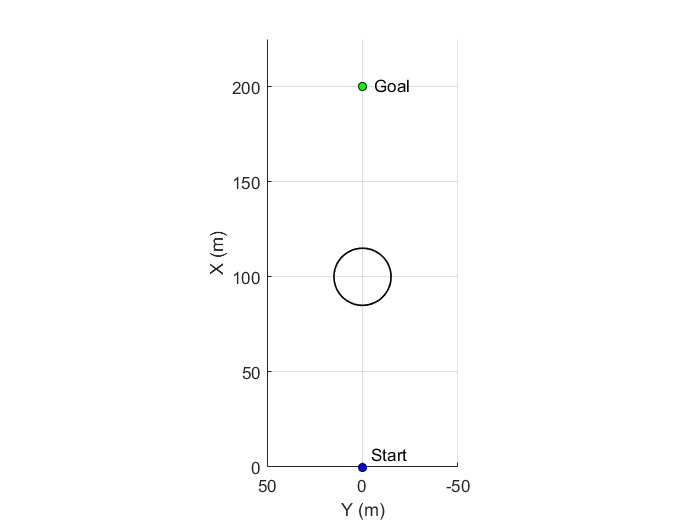
\includegraphics[width=\columnwidth]{Figs/ObstacleField1.png}
	\caption{\small Obstacle Field 1}  
	\label{fig:Obst1}
\end{figure}

\begin{table}
\begin{center}
	\begin{tabular}{||c|c|c|c||} 
		\hline
		& x & y & Radius\\
		\hline
		Target Location  & 200.0 & 0.0 & -\\ 
		\hline
		Obstacle 1 & 100.0 & 0.0 & 15.0\\
		\hline
	\end{tabular}
\end{center}
\caption{Obstacle Field 1 Summary}
\label{t:Obst1Summary}
\end{table}

\begin{figure}
	\centering
	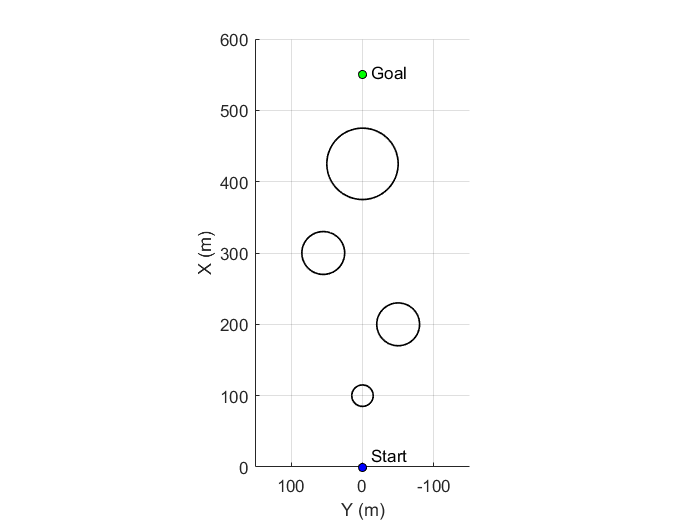
\includegraphics[width=\columnwidth]{Figs/ObstacleField2.png}
	\caption{\small Obstacle Field 2}   
	\label{fig:Obst2}
\end{figure}

\begin{table}
\begin{center}
	\begin{tabular}{||c|c|c|c||} 
		\hline
		& x & y & Radius\\
		\hline
		Target Location  & 550.0 & 0.0 & -\\ 
		\hline
		Obstacle 1 & 100.0 & 0.0 & 15.0\\
		\hline
		Obstacle 2 & 200.0 & -50.0 & 30.0\\
		\hline
		Obstacle 3 & 300.0 & 55.0 & 30.0\\
		\hline
		Obstacle 4 & 425.0 & 0.0 & 50.0\\
		\hline
	\end{tabular}
\end{center}
\caption{Obstacle Field 2 Summary}
\label{t:Obst2Summary}
\end{table}

For this paper two obstacle fields were generated. The first contains one large circular obstacle located along the initial heading of the vehicle. The target position is located a large distance behind the single obstacle. Figure~\ref{fig:Obst1} presents this obstacle field. The goal of this test is to analyze the performance of the vehicle and controller around a single obstacle. 

The second obstacle field contains four circular obstacles of varying sizes placed in the vehicle’s initial heading direction. The performance of the vehicle on this obstacle field should allow for understanding of how the controller and vehicle navigate around multiple obstacles in a more realistic scenario. Refer to Fig.~\ref{fig:Obst2}.

The following vehicle parameters are maintained throughout all of the executed tests. A PID speed controller is used to maintain a near constant speed of 8.1 m/s longitudinally for the simulated plant {\CHRONO} wheeled vehicle. This constant speed is enforced in the analytical models internal to the MPC local obstacle avoidance controller. The LIDAR sensor has a maximum range $R_{LIDAR}$ of 129.6 meters and is sampled instantaneously at increments of $2.5^\circ$. The vehicle is limited to a maximum steering angle of $10^\circ$ with a maximum steering rate of  $70.63^{\circ}/s$. 

%% ============================================================

\section{SIMULATION RESULTS}\label{s:results}

This section summarizes the results of the four tests listed in Table~\ref{t:TestMatrix}. 

\begin{figure}
	\centering
	\begin{subfigure}[b]{\columnwidth}
		\centering
		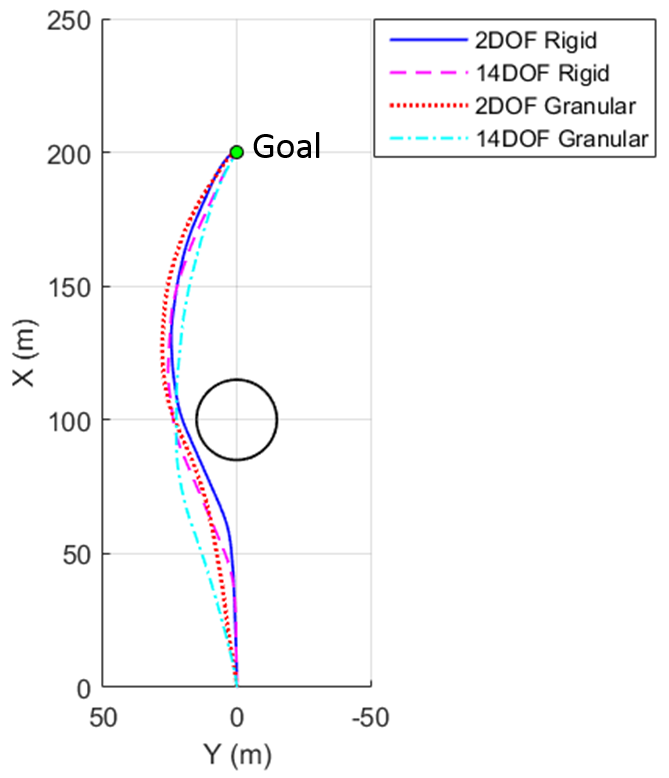
\includegraphics[width=\columnwidth]{Figs/ObstacleField1Trajectories.png}
		\caption{{\small Trajectories from Tests on Obstacle Field 1}}   
		\label{fig:ObstacleField1Trajectories}
	\end{subfigure}
	\hfill
	\begin{subfigure}[b]{\columnwidth}
		\centering
		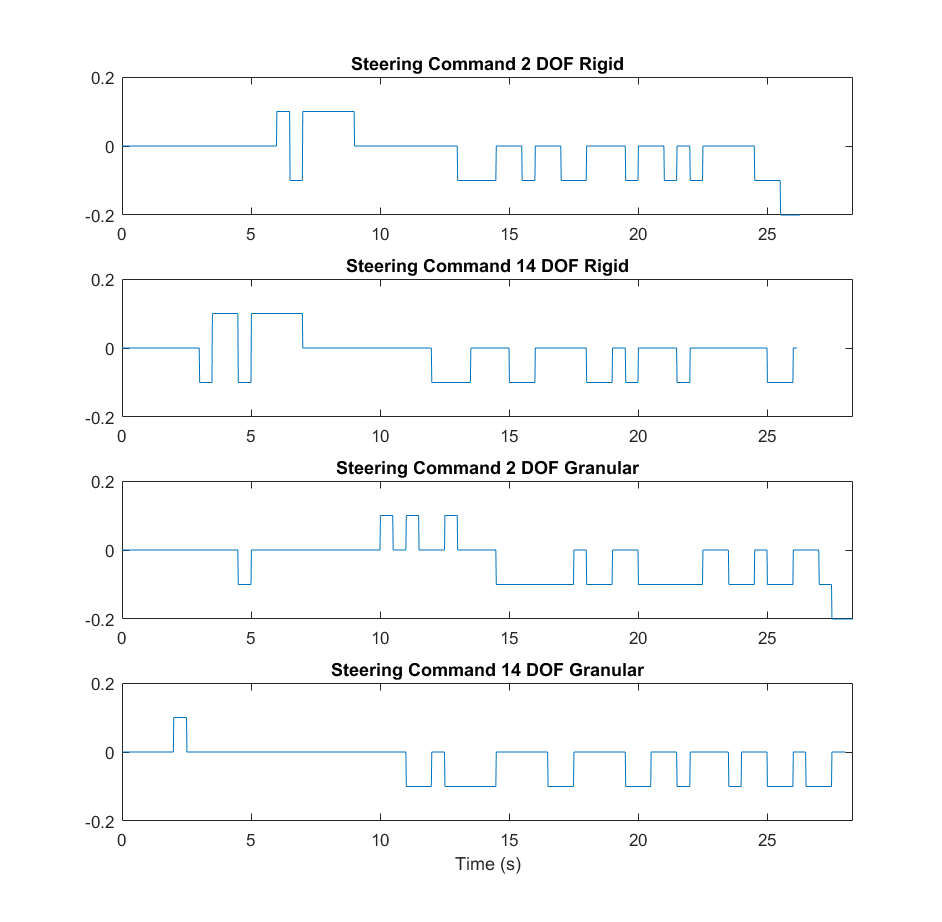
\includegraphics[width=\columnwidth]{Figs/SteeringCommandsField1.png}
		\caption{\small Steering Commands on Obstacle Field 1}   
		\label{fig:SteeringCommandsField1}
	\end{subfigure}
	\caption{\small Trajectories and Steering Data for Obstacle Field 1}
	\label{fig:Obst1TestData}
\end{figure}

\begin{table*}
		\centering
\begin{tabular}{ ||p{5cm}|p{2cm}|p{2cm}|p{2cm}|p{2cm}||  }
		\hline
		Test Number & 1 & 2 & 3 & 4\\
		\hline
		Controller Model & 2-DOF & 14-DOF & 2-DOF & 14-DOF\\
		\hline
		Terrain & Rigid & Rigid & Granular & Granular\\
		\hline
		Time to Target (s)  & 26.67 & 26.15 & 28.32 & 28.03\\ 
		\hline
		Minimum Obstacle Distance (m) & 0.897 & 5.462 & 3.491 & 4.721\\
		\hline
		Controller Effort & 0.0340 & 0.0340 & 0.0340 & 0.0306\\
		\hline
		Max Lateral Acceleration (m/s$^{2}$)& 2.78 & 1.57 & 2.47 & 2.33 \\
		\hline
		Average Lateral Acceleration (m/s$^{2}$) &0.54 & 0.51 & 0.55 & 0.46\\
		\hline
\end{tabular}
\caption{Test Evaluation Metrics Summary on Obstacle Field 1}
\label{t:EvalMetricsObst1}
\end{table*}






\begin{figure}
	\centering
	\begin{subfigure}[b]{\columnwidth}
		\centering
		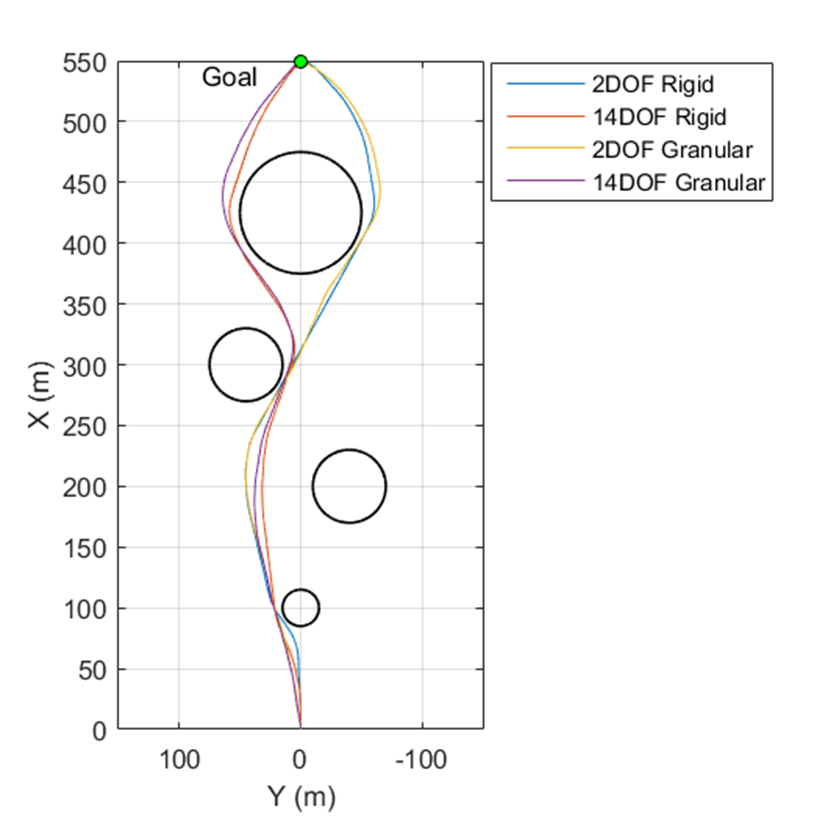
\includegraphics[width=\columnwidth]{Figs/ObstacleField2Trajectories.png}
		\caption{{\small Trajectories from Tests on Obstacle Field 2}}   
		\label{fig:ObstacleField2Trajectories}
	\end{subfigure}
	\hfill
	\begin{subfigure}[b]{\columnwidth}
		\centering
		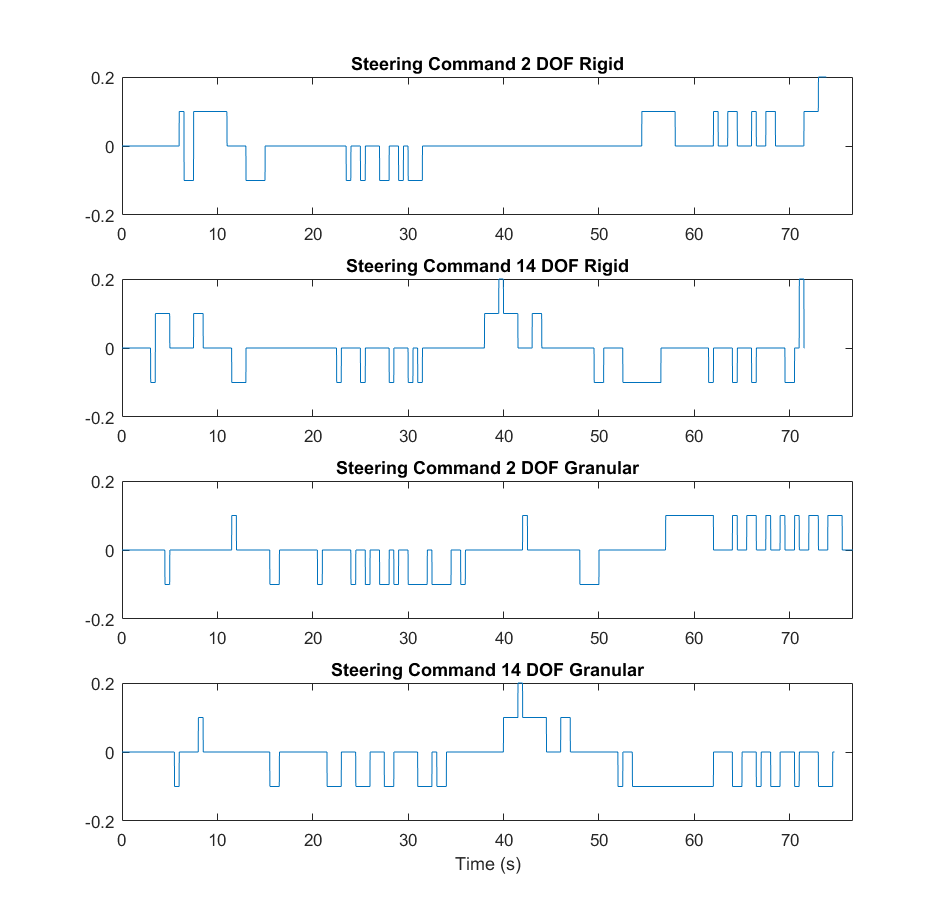
\includegraphics[width=\columnwidth]{Figs/SteeringCommandsField2.png}
		\caption{\small Steering Commands on Obstacle Field 2}   
		\label{fig:SteeringCommandsField2}
	\end{subfigure}
	\caption{\small Trajectories and Steering Data for Obstacle Field 2}
	\label{fig:Obst2TestData}
\end{figure}

\begin{table*}
		\centering
\begin{tabular}{ ||p{5cm}|p{2cm}|p{2cm}|p{2cm}|p{2cm}||  }
		\hline
		Test Number & 1 & 2 & 3 & 4\\
		\hline
		Controller Model & 2-DOF & 14-DOF & 2-DOF & 14-DOF\\
		\hline
		Terrain & Rigid & Rigid & Granular & Granular\\
		\hline
		Time to Target (s)  & 73.85 & 71.55 & 76.64 & 74.70\\ 
		\hline
		Minimum Obstacle Distance (m) & 0.331 & 2.599 & 1.083 & 1.152\\
		\hline
		Controller Effort & 0.0510 & 0.0680 & 0.0714 & 0.0612\\
		\hline
		Max Lateral Acceleration (m/s$^{2}$)& 2.92 & 2.51 & 2.55 & 2.45 \\
		\hline
		Average Lateral Acceleration (m/s$^{2}$) & 0.41 & 0.43 & 0.53 & 0.58\\
		\hline
\end{tabular}
\caption{Test Evaluation Metrics Summary on Obstacle Field 2}
\label{t:EvalMetricsObst2}
\end{table*}

The trajectories for the four performed tests are presented in Fig. \ref{fig:ObstacleField1Trajectories} on Obstacle Field 1 and Fig. \ref{fig:ObstacleField2Trajectories}  on Obstacle Field 2 and their associated steering commands generated by the controller are presented in Fig. \ref{fig:SteeringCommandsField1} and \ref{fig:SteeringCommandsField2}. Just from looking at the trajectories of the vehicles, several observations can be made. The controlled vehicle in each test successfully maneuvers around the single obstacle in Obstacle Field 1. From this we can see as has been proven in~\cite{ModelFidelity2016} that even though the 2-DOF yaw plane vehicle model lacks the complexity and fidelity of the 14-DOF model, it can still safely navigate a vehicle successfully through an obstacle field while moving at a non-extreme speed. The evaluation metrics for each test as defined in Section~\ref{ss:Metrics} are tabulated for the runs on each obstacle field. The evaluation metrics for the runs on Obstacle Field 1 are presented in Table~\ref{t:EvalMetricsObst1} and for Obstacle Field 2 in Table~\ref{t:EvalMetricsObst2}. 

Comparing the results of Test 1 and Test 2, we are able to examine the performance differences that occur when a 2-DOF internal vehicle model is used within the controller to control the {\CHRONO} vehicle as opposed to the higher fidelity 14DOF internal vehicle model used in the controller in Test 2. On both Obstacle Field 1 and 2, the controllers that use the 14-DOF internal vehicle model to predict vehicle states guides the {\CHRONO} vehicle to the goal quicker than the controllers with the internal 2DOF vehicle model. However, in each of these instances the time difference is slim. At most in these tests a controller using the 14DOF internal vehicle reaches the target 2.2 seconds faster than the 2DOF controller tests. So in this regard the 14DOF controllers perform marginally better than the 2DOF controllers. One area the 2-DOF controller model of Test 1 performs better than the 14-DOF model of Test 2 is in the minimum Obstacle Distance
metric. In all the cases, the controllers with the 2-DOF internal vehicle model guided the vehicle closer to the obstacles than the controllers with the 14-DOF models. This is a desirable characteristic in that the 2-DOF controllers are taking more advantage of the controlled vehicle's dynamic capabilities when navgiating around obstacles. Comparing the controller effort between Tests 1 and 2, on Obstacle Field 1 the controller effort is actually the same. The 2-DOF controller does input more command changes than the 14-DOF controller. On Obstacle Field 2, the 14-DOF controller of Test 2 actually has a higher controller effort value than the 2-DOF controller by 0.0170. This may however be due to the controller's decision to move left around the last obstacle instead of continueing straight around the right side of the obstacle as the 2-DOF controller commands. Finally looking at the maximum and average lateral accelerations between test 1 and test 2, regarding both of these metrics  the 14-DOF controller performs better than the 2-DOF controller on rigid terrain. Overall looking at all these metrics, on rigid terrain the 14-DOF controller performs marginally better than the 2-DOF controller. However considering the 14-DOF takes much longer to run and the fact that realtime implementation of a model predictive controller with internal 14-DOF vehicle model would be less feasible, the 2-DOF is suitable for use in an MPC local obstacle avoidance controller for a vehicle on rigid ground terrain traveling at non-extreme speeds. The performance drop is slight switching to the 2-DOF vehicle model, but can still safely navigate the vehicle around an obstacle field to an end goal. These results support the findings and conlusions of~\cite{ModelFidelity2016} on a different AGV. 

The same set of comparisons are made between the 2-DOF controller and the 14-DOF controller but now on granular terrain in Tests 3 and 4. Similar to rigid ground, the 14-DOF controller navigates the {\CHRONO} vehicle to the specified end goal quicker than the 2-DOF controller at most by 1.94 seconds. Again though, this time difference is marginal so even though the 14-DOF controller performs better than the 2-DOF controller regarding time to target, this does not mean at all that the 2-DOF controller performs poorly. On Obstacle Field 1 and Obstacle Field 2, the 2-DOF controller guides the vehicle closer to obstacles on granular terrain than the 14-DOF controllers. The 14-DOF controller has a lower controller effort value than the compared 2-DOF controller on granular terrain in Tests 3 and 4. Finally looking at the maximum and average lateral accelerations between Tests 3 and 4, on Obstacle Field 1 the 2-DOF has a higher maximum lateral acceleration and average lateral acceleration. On Obstacle Field 2 the 2-DOF controller results in a lower maximum lateral acceleration and average lateral acceleration than the 14-DOF controller of test 4 on granular terrain. Overall looking at the previously mentioned metrics, the 14-DOF controller again performs marginally better than the 2-DOF controller on granular terrain. Even though the 2DOF and 14DOF internal vehicle models were derived using rigid ground assumptions, they are still capable of successfully navigating the {\CHRONO} vehicle through an obstacle field safely on certain granuler media. The same conclusion from this comparison can be made as from comparing Tests 1 and 2. Though vehicle performance marginally drops when using the 2-DOF controller, realistically the software benefits of using the 2-DOF controller outweigh the slight performance drop seen by this study at non-extreme vehicle speeds.

By comparing Tests 2 and 4, observations are made about the difference between a vehicle operating on rigid ground versus granular terrain when the controller is held constant. In this case, the controller used is the 14-DOF controller so we can analyze performance differences between navigating on rigid ground versus granular terrain. In all cases the time to target is lower on rigid ground tests than on granular tests we will ignore that evaluation metric when making the comparison between Tests 2 and 4. In Test 4, the vehicle navigates much closer to any obstacle than in Test 2 on rigid ground. On granular terrain though, the controller effort is lower than on rigid ground. Comparing the lateral acceleration metrics of Tests 2 and 4 yield no discernable conclusions since neither is significantly nor consistently larger than the other in either of the tests. Comparing Tests 1 and 3 yields similar conclusions as comparing Tests 2 and 4. On rigid ground, the 2-DOF controller does a better job of approaching the obstacles more closely. The controller effort is also lower in Test 1 on rigid ground than on granular terrain in Test 3.

Just from looking at the lateral accelerations, we see the forces the vehicle experiences from driving on granular terrain can be much different than forces on simple rigid ground. Even examining Figs.~\ref{fig:ObstacleField1Trajectories} and \ref{fig:ObstacleField2Trajectories}, the vehicle navigating on granular terrain does not turn as sharply for a given steering command as the vehicle does on rigid ground terrain. To really understand the differing behavior between a vehicle driving on rigid terrain to a vehicle driving on granular terrain, a parametric study should be performed analyzing the vehicle driving on a variety of granular terrain with different granular parameters. 

%% ============================================================

\section{CONCLUSIONS}\label{s:conclusion}

In this study, using the multibody physics API {\CHRONO} a simulation has been developed of a HMMWV driving through a user specified obstacle field towards a defined target location. Within this simulation, a MPC LIDAR based local obstacle avoidance controller has been implemented to navigate the vehicle around obstacles as it encounters them. The controller itself uses a simplified analytical vehicle model to predict the actual controlled {\CHRONO} vehicle states within a finite prediction horizon in order to determine the optimal path and steering sequence forward from the current vehicle state. A method of simulating granular terrain for this large obstacle field was developed and implemented for this study. Two separate MPC Algorithms were developed, one that uses a 2-DOF vehicle model to predict {\CHRONO} vehicle states and a 14-DOF model to do the same. These two controllers were used to navigate a {\CHRONO} HMMWV through two obstacle courses on both rigid terrain and then on granular terrain. The results were compared to understand what if any improvements need to be made to the MPC LIDAR based local obstacle avoidance controller to successfully control a vehicle on granular terrain. 

As in \cite{ModelFidelity2016}, the controller with the 14-DOF internal vehicle model performs marginally better than the controller with the 2-DOF internal vehicle model in all situations. However, tests with the 2-DOF controller prove that this controller can still successfully navigate a vehicle through an obstacle field when the vehicle is moving at non-extreme speeds. Using the 2-DOF controller also allows for faster calculation of optimal steering sequences which is required for eventual realtime implementation. Both of the controllers navigated the vehicle worse on granular terrain than on rigid ground terrain, but this is expected since the internal vehicle controller models were derived using rigid ground assumptions. This study also highlights the complexities introoduced to vehicle modeling when the terrain is no longer rigid. Looking at the vehicle trajectories and lateral accelerations on granular terrain, there are clear differences in tire ground interactions when the terrain is now granular. The terrain granular parameters affect the turning characteristics of the vehicle, acceleration abilities, and overall vehicle dynamic performance which is not control predictive with the currently used 2-DOF and 14-DOF analytical vehicle models. 

The results of this study are promising. Since the 2-DOF controller is able to navigate the {\CHRONO} vehicle on this study's granular terrain, then there is some small set of granular terrain on which a 2-DOF model is sufficient for predicting vehicle performance well enough to guide the vehicle successfully and safely to a target point. However, these results also emphasize the need for future research and studies relating to vehicle simulation on granular terrain. This same sort of study should be performed parametrically on a comprehensive set of different granular terrains to understand the difference between vehicle performance on rigid ground and granular terrain. From there, a new intermediate analytical model should be research and developed that is not as complex as the 14-DOF model but does take into account granuler parameters such as the friction angle. 

%% ============================================================

\section*{Acknowledgments}
{\CHRONO} development was supported in part by U.S. Army TARDEC Rapid Innovation Fund grant No. W911NF-13-R-0011, Topic No. 6a, ``Maneuverability Prediction''.
Support for the development of {\ChronoVehicle} was provided by U.S. Army TARDEC grant W56HZV-08-C-0236.

%% ============================================================

\bibliographystyle{unsrt}
\bibliography{references}

%% ============================================================


\end{document}



